\documentclass[11pt]{article}

\usepackage[T1]{fontenc}
\usepackage[utf8]{inputenc}
\usepackage{lmodern}
\usepackage[margin=2.4cm]{geometry}
\usepackage{graphicx}
\graphicspath{{figures/}}
\usepackage{booktabs}
\usepackage[hidelinks,unicode]{hyperref}
\usepackage{microtype}

\hypersetup{
  pdftitle={How close a from-scratch GPT-2 gets to a Tesla T4},
  pdfauthor={Danilo Nikić}
}

\title{How close a from-scratch GPT-2 gets to a Tesla T4}
\author{Danilo Nikić\\
Department of Mathematics and Informatics,\\
Faculty of Sciences, University of Novi Sad, Serbia\\
nikicdanilo06@gmail.com\\
dmi.75.24@student.pmf.uns.ac.rs}
\date{November 15, 2026}

\begin{document}
\maketitle

\begin{abstract}
A from-scratch GPT-2 training step in C++ and CUDA keeps its FP32 path.
On a Tesla T4, a tiled GEMM reaches 31\% of the published FP32 peak (8.1~TFLOP/s) and cuBLAS reaches 52\%, both on a $1024^3$ product.
A first tensor-core kernel, FP16 inputs with FP32 accumulation, reaches 3.3\% of the 65~TFLOP/s FP16 tensor peak and is slower than both FP32 kernels at that size.
At the shipped context of 64, attention, softmax, and the small products are launch-bound.
At context 1024, scored attention and softmax sit on the memory side of the roofline, and a fused attention kernel is faster only once the score matrix no longer fits in cache.
\end{abstract}

\noindent Code: \url{https://github.com/damnilo/GPT-2-From-Scratch-Cpp}

\section{Motivation and related work}

The question is how much of a T4 the from-scratch FP32 training step and the inference kernels measured beside it can reach, and which operation limits them as the context grows.
The shipped model is small on purpose: width 32, four heads, three blocks, context 64, vocabulary 5256, batch size 1.
The training step that keeps the embeddings and the block on the device measures 5.755~ms with cuBLAS at that width.
Inference kernels are measured beside that path. They do not replace it.

FlashAttention computes the same masked softmax attention without writing the score matrix, by tiling the query and keeping a running maximum and sum~\cite{flash}.
The fused kernel here is that idea at a smaller scale: one thread owns one query row, tiles are 64, and the score matrix is not allocated.
It is an inference measurement. Training attention still stores the scores, because the backward pass reads them.
llm.c is a GPT-2 implementation in C with CUDA training~\cite{llmc}.
This repository is in the same spirit and much smaller. It does not load the 124M public weights and does not report WikiText perplexity.
cuBLAS is the vendor GEMM used as the FP32 reference~\cite{cublas}.
The roofline model is how the times are read: arithmetic intensity against a compute roof and a bandwidth roof~\cite{roofline}.

\section{Method}

Host code is C++20. CUDA files are C++17.
Measurements were collected on Google Colab, on a Tesla T4 (compute capability 7.5, 15~GB) with NVIDIA driver 580.82.07 and CUDA 13.0 (nvcc V13.0.88).
Every timed cell is two warmups and then the median of ten repeats.
The peaks used as roofs are the published T4 rates: 8.1~TFLOP/s FP32, 65~TFLOP/s FP16 tensor-core, and 320~GB/s.
A cell under 0.05~ms is marked launch. Its percent of peak is not a throughput result.
Bytes are compulsory traffic: each input is read once and each output is written once, unless the kernel's loop says otherwise.
They are not DRAM counters from Nsight Compute.

The FP32 GEMM has two device implementations.
cuBLAS is called on row-major operands by swapping the arguments.
The tiled kernel uses a $64 \times 64$ output tile, a K strip of 16, and a $4 \times 4$ register tile per thread.
When the dimensions divide those tiles, a second kernel drops the edge checks.
The cutoff that sends a host tensor product to cuBLAS stays at a dimension product of 65536, and the tile stays 64.
Training uses cuBLAS when the head width is not a multiple of 16.
The shipped head width is 8, so the training step selects cuBLAS.
\texttt{generate} stays on the tiled kernel.

Fused attention covers the middle of the forward only: the score product, the causal softmax, and the product with $V$.
The Q, K, and V projections and the output projection stay outside.
Online softmax keeps a running maximum $m$ and a running sum $\ell$.
A new tile rescales the accumulator by $\exp(m - m')$ before adding the new weighted values.
Keys after the query position are masked to $-\infty$.
The kernel rejects a head width above 32, because the query row lives in registers.

The tensor-core GEMM is a separate function, \texttt{wmmaGemmDevice}.
Inputs are rounded from FP32 to FP16 before the timed region.
Each warp computes a $16 \times 16$ output tile with WMMA, accumulating in FP32.
Rows, the shared dimension, and columns must be multiples of 16, so the shipped head width of 8 is rejected.
The FP32 training and generate paths do not call it.

\section{Experiments}

\subsection{Matrix product}

On the $1024^3$ product the tiled kernel is at 31\% of the FP32 roof and cuBLAS at 52\%.
Both sit above the FP32 ridge (about 25~FLOP/byte; the product's intensity is 171), so the roofline in Figure~\ref{fig:roofline} calls them compute-bound.
The WMMA kernel's intensity is 256~FLOP/byte, above the tensor ridge, but it delivers 2160~GFLOP/s, 3.3\% of 65~TFLOP/s, and 0.994~ms against 0.515~ms for cuBLAS.
The kernel loads each WMMA fragment from global memory and caps the grid at 128 blocks.
That is a correct tensor-core product, not a kernel that occupies the machine.
At the feed-forward shapes of the shipped model ($64 \times 32 \times 128$ and $64 \times 128 \times 512$) every GEMM finishes between 0.011~ms and 0.035~ms.
Those cells are launch, which is why a tensor-core kernel can look fastest there and still be the slow one at $1024^3$.
Against FP32 cuBLAS, the WMMA absolute error on the small shapes is $2 \times 10^{-5}$ to $6 \times 10^{-5}$.

\begin{figure}[t]
  \centering
  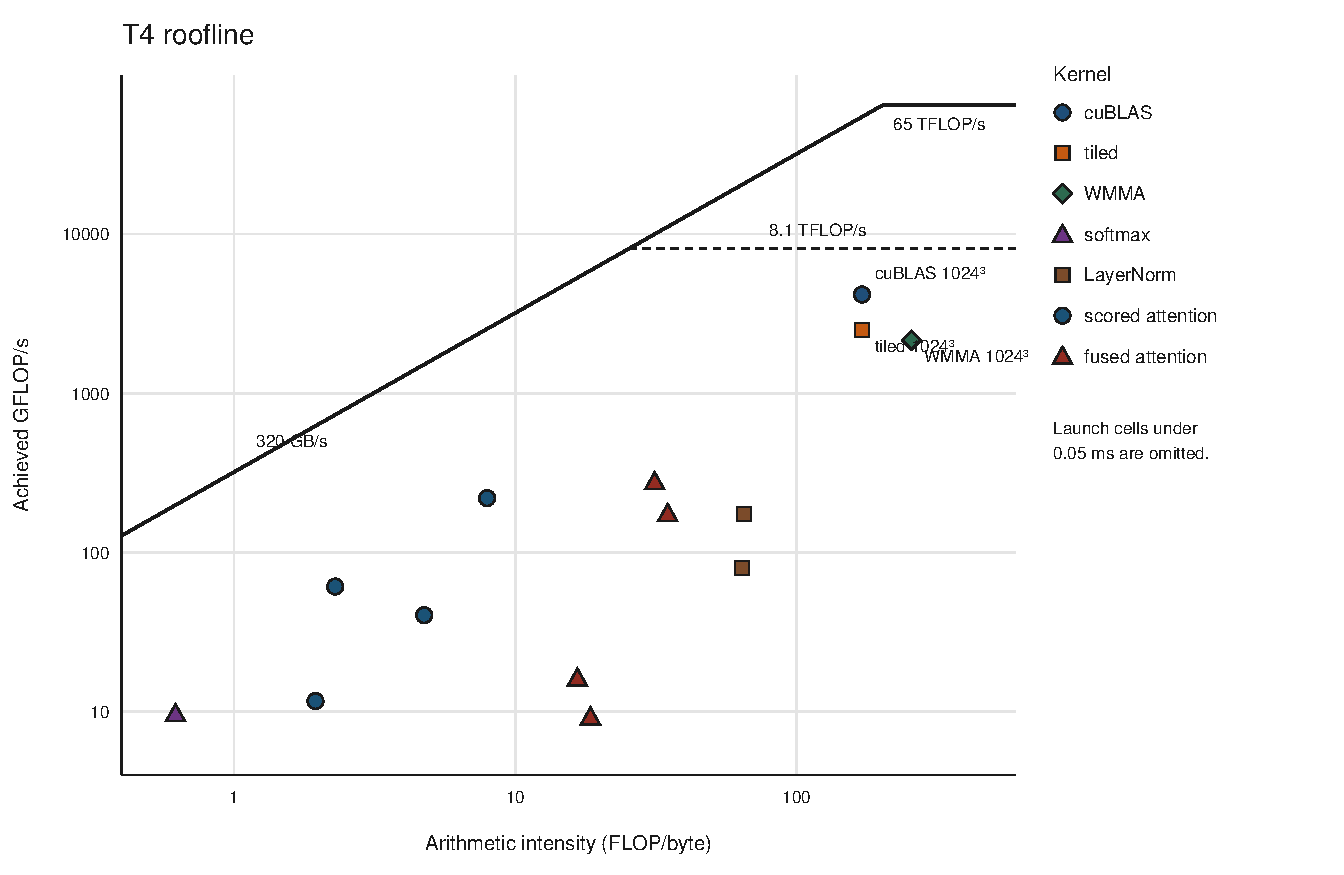
\includegraphics[width=\linewidth]{roofline.pdf}
  \caption{T4 roofline from compulsory traffic. Launch cells under 0.05~ms are omitted. The solid line is 320~GB/s, breaking to the 65~TFLOP/s tensor roof. The dashed line is the 8.1~TFLOP/s FP32 roof.}
  \label{fig:roofline}
\end{figure}

\subsection{Attention, softmax, and LayerNorm}

Figure~\ref{fig:latency} is the scored path (cuBLAS) against fused attention, four heads, head widths 8 and 32.
The scored path writes an $H \times T \times T$ score matrix.
At $T = 64$ that matrix is 64~KiB and fused attention is slower: 0.082~ms against 0.063~ms at head width 8, and 0.171~ms against 0.068~ms at head width 32.
At $T = 1024$ the score matrix is 16~MiB. Fused attention at head width 8 is 1.166~ms and the scored cuBLAS path is 3.259~ms.
At head width 32 the gap is smaller, 1.551~ms against 1.783~ms.
A second run, inside the roofline program, goes the same way at head width 8: fused 0.881~ms, scored 2.538~ms.

The roofline says why.
Scored attention at $T = 1024$ has intensity 2.3~FLOP/byte (head width 8) and 7.9 (head width 32), under the FP32 ridge, and moves about 27~GB/s, near 9\% of the memory roof.
Fused attention drops the score matrix, so the intensity rises to about 31--35~FLOP/byte and the point is labeled compute.
The kernel is still one thread per query row, so the achieved rate is 176~GFLOP/s and 278~GFLOP/s, a few percent of the FP32 roof.
Fused attention wins on time at long context because it moves less data, not because it fills the GPU.

Masked softmax at $T = 1024$ and four heads takes 2.156~ms by itself, with intensity 0.62~FLOP/byte.
One thread walks one row.
That single kernel is in the same range as the whole scored attention.
LayerNorm at $T = 1024$ and width 128 takes 0.391~ms and is labeled compute because every channel thread repeats the mean and the variance.
The achieved rate is 174~GFLOP/s. The label describes the redundant loop, not a kernel that is close to the roof.

\begin{figure}[t]
  \centering
  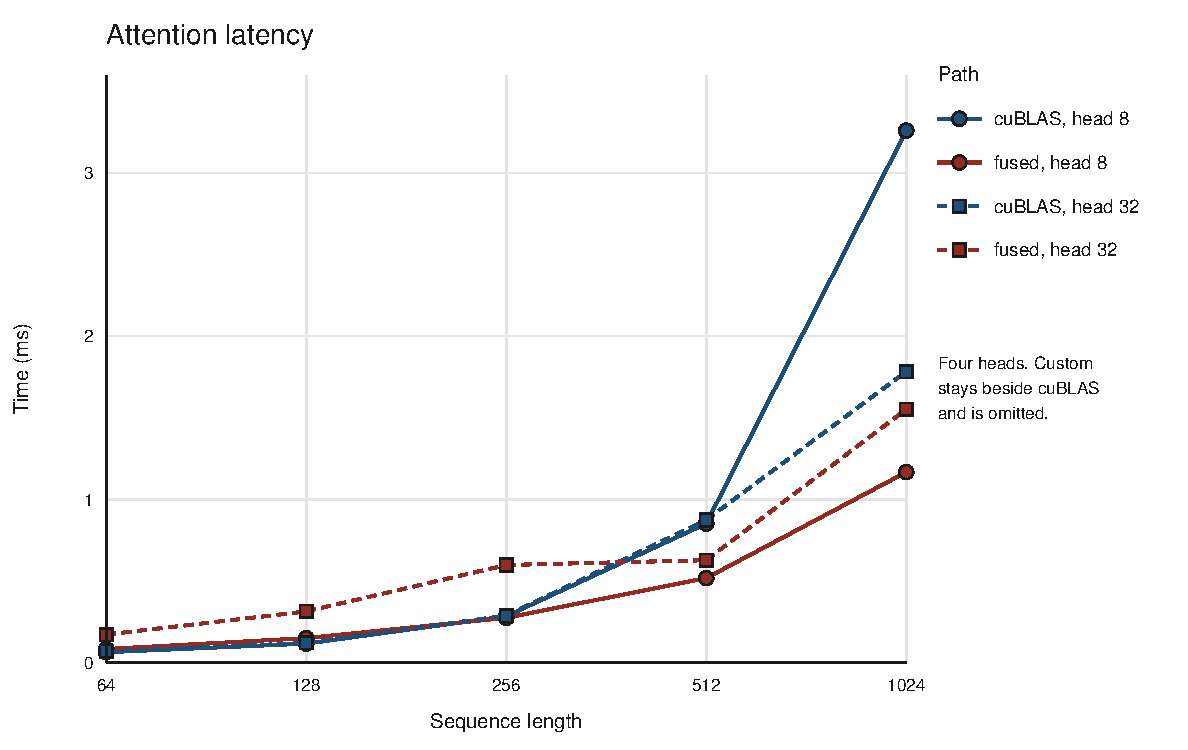
\includegraphics[width=0.92\linewidth]{attention_latency.pdf}
  \caption{Attention latency against sequence length, four heads. Blue is the scored cuBLAS path. Red is fused attention. Solid lines are head width 8, dashed lines head width 32. The custom GEMM stays beside cuBLAS and is omitted.}
  \label{fig:latency}
\end{figure}

\section{Limitations and future work}

The tensor-core path does not belong in the training step.
At the one size large enough to leave kernel launch, it is slower than FP32 cuBLAS and far from the tensor roof.
A shared-memory WMMA kernel, without the 128-block cap, is the change that would test whether the T4 tensor cores are reachable from this codebase.
The T4 has no BF16 tensor cores, so that experiment stays FP16 with FP32 accumulation.
Head width 8 cannot enter it without padding.

Fused attention does not belong in \texttt{generate} or in the training backward.
At context 64 it is slower, and the backward pass still needs the stored scores.
\texttt{generate} also restarts positions at 0 when the context window slides, so a cache of past keys and values would not match the sampler.
Nsight Compute was not collected. Colab often refuses the GPU counters.
The roofline bytes would move if the measured DRAM traffic were higher than the compulsory count.
The public GPT-2 weights of 124M, and a WikiText-2 perplexity, are a different model from the one measured here.

\section{Conclusion}

On a $1024^3$ product the tiled FP32 kernel reaches 31\% of the T4's published FP32 peak and cuBLAS reaches 52\%, while the first WMMA kernel reaches 3.3\% of the tensor peak and is slower than both.
At the shipped context of 64, attention, softmax, and the small products are launch-bound.
At $T = 1024$, fused attention is faster because it moves less data, not because it fills the GPU.
A shared-memory WMMA kernel, without the 128-block cap, is the next test of whether the T4 tensor cores are reachable from this codebase.

\begin{thebibliography}{9}
\bibitem{flash}
Tri Dao, Daniel~Y. Fu, Stefano Ermon, Atri Rudra, and Christopher R\'e.
FlashAttention: Fast and Memory-Efficient Exact Attention with IO-Awareness.
\emph{Advances in Neural Information Processing Systems}, 2022.

\bibitem{llmc}
Andrej Karpathy.
llm.c.
\url{https://github.com/karpathy/llm.c}.

\bibitem{cublas}
NVIDIA.
cuBLAS.
\url{https://docs.nvidia.com/cuda/cublas/}.

\bibitem{roofline}
Samuel Williams, Andrew Waterman, and David Patterson.
Roofline: An Insightful Visual Performance Model for Multicore Architectures.
\emph{Communications of the ACM}, 52(4):65--76, 2009.
\end{thebibliography}

\end{document}
